\chapter{Implementation}
We implemented our system on a network of phones, with no servers. Every mobile phone cooperates by sharing music and establishing trust. This means that the computational capacity grows with the amount of users, as does the demand on such capacity. The system is built along the ideologies of a DAO: there is no single party, server or database that the system requires to operate. As such, it is a non-profit system, where the artists keep all revenues. In MusicDAO, mobile phones are able to transfer money and music. In this trustless system, trust in other parties is established through proofs of identity using cryptography, and publicly verified append-only history data. It is resilient against censorship-attacks: it cannot be taken down by any government or institution. The main features of our work in comparison to the state-of-the-art related work (see sec. \ref{sec:related-work}) can be viewed in table \ref{tab:comparison}. The most notable components of MusicDAO are visualized in fig.  \ref{fig:main-components}.
\\
\\
\textbf{Features overview}
\begin{itemize}
    \item Defining digital musical releases using metadata, and sharing those with peers;
    \item Immutable storage of music metadata and cryptographic identification of artists;
    \item Peer-to-peer music streaming over BitTorrent; Prioritization algorithm to minimize streaming latency; Caching of audio files and metadata.
    \item Browsing playlists; Local and remote keyword search for music.
    \item Mobile Bitcoin wallet implementation; Peer-to-peer donations to artists using Bitcoin.
    \item A content popularity gossip-based algorithm.
\end{itemize}
The following was not implemented:
\begin{itemize}
    \item Artist Income Division Algorithm.
\end{itemize}
Apart from the Android SDK and the TrustChain Superapp, the main libraries that are used are JLibtorrent\footnote{\url{https://github.com/frostwire/frostwire-jlibtorrent}} (Libtorrent protocol interface), BitcoinJ\footnote{\url{https://bitcoinj.org/}} (Bitcoin protocol interface) and ExoPlayer\footnote{\url{https://github.com/google/ExoPlayer}} (Android media player). 

The Artist Income Division Algorithm, presented in the Design chapter, is not implemented in MusicDAO at the time of writing. However, the implementation does provide the critical component of this algorithm: an integration with peer-to-peer direct donations without intermediaries. As such, AIDA can be trivially implemented by another researcher or developer.

\begin{figure}
    \centering
    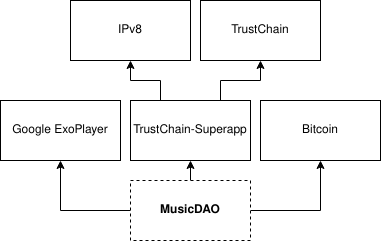
\includegraphics[width=0.45\textwidth]{implementation/simplified-components.png}
    \caption{The main external components used in MusicDAO}
    \label{fig:main-components}
\end{figure}

\begin{table}[]
\begin{tabular}{|l|l|l|l|l|}
\hline
\textbf{}         & Transparent revenue streams & Self-governance & \textgreater{}99.99\% to artists & Fully P2P, self-scaling \\ \hline
Audius            & \Checkmark & \Checkmark                                 & $\times$                        & $\times$                                 \\ \hline
Musicoin          & \Checkmark & $\times$                                & $\times$                        & $\times$                                   \\ \hline
Opus Audio        & \Checkmark & \Checkmark                                & $\times$                        & $\times$                                  \\ \hline
\textbf{MusicDAO} & \CheckmarkBold &  $\times$                       &  \CheckmarkBold                       &  \CheckmarkBold     \\ \hline
\end{tabular}
\caption{Overview of work implemented in this thesis compared to related work (see sec. \ref{sec:related-work})}
\label{tab:comparison}
\end{table}

\section{Zero-server infrastructure Android application}
The system described in chap. \ref{chap:design} is implemented on a network of phones, with no servers. This results in a fully distributed, leaderless organization. Every mobile phone cooperates by sharing music, transacting money and establishing trust. This means that the computational capacity grows with the amount of users, as does the demand on such capacity. The system is built along the ideologies of a DAO: there is no single party, server or database that the system requires to operate. As such, it is a non-profit system, where the destination of money flow is decided by its users, instead of by a single organization. In MusicDAO, mobile phones are able to transfer money and music. In this trust-less system, trust in other parties is established through proofs of identity using cryptography, and publicly verified using append-only history data.

MusicDAO is an Android application which runs on any Android device running version 5.1.1 or above. It is implemented as a `mini-app' of the \textit{TrustChain Superapp}~\citep{mattskala2020}. This follows the concept of super apps~\citep{kpmg2019superapps}. The app is published on the Android Play Store\footnote{\url{https://play.google.com/store/apps/details?id=nl.tudelft.trustchain}} and runs on Android 5.1 and above. Its code is publicly available\footnote{\url{https://github.com/Tim-W/trustchain-superapp}}. As programming language Kotlin is selected, as it is the preferred language for Android development\footnote{\url{https://android-developers.googleblog.com/2019/05/google-io-2019-empowering-developers-to-build-experiences-on-Android-Play.html}}. Moreover the underlying technology stack is also written in Kotlin, so this allows for neat integration. This section describes the implementation choices, usage of external libraries and presents the user interface of MusicDAO. The main interfaces of the app can be seen below (figs. \ref{fig:screenshot-home}, \ref{fig:screenshot-playlist} and \ref{fig:tip-artist}).

\begin{figure}[]
    \minipage{0.3\textwidth}
        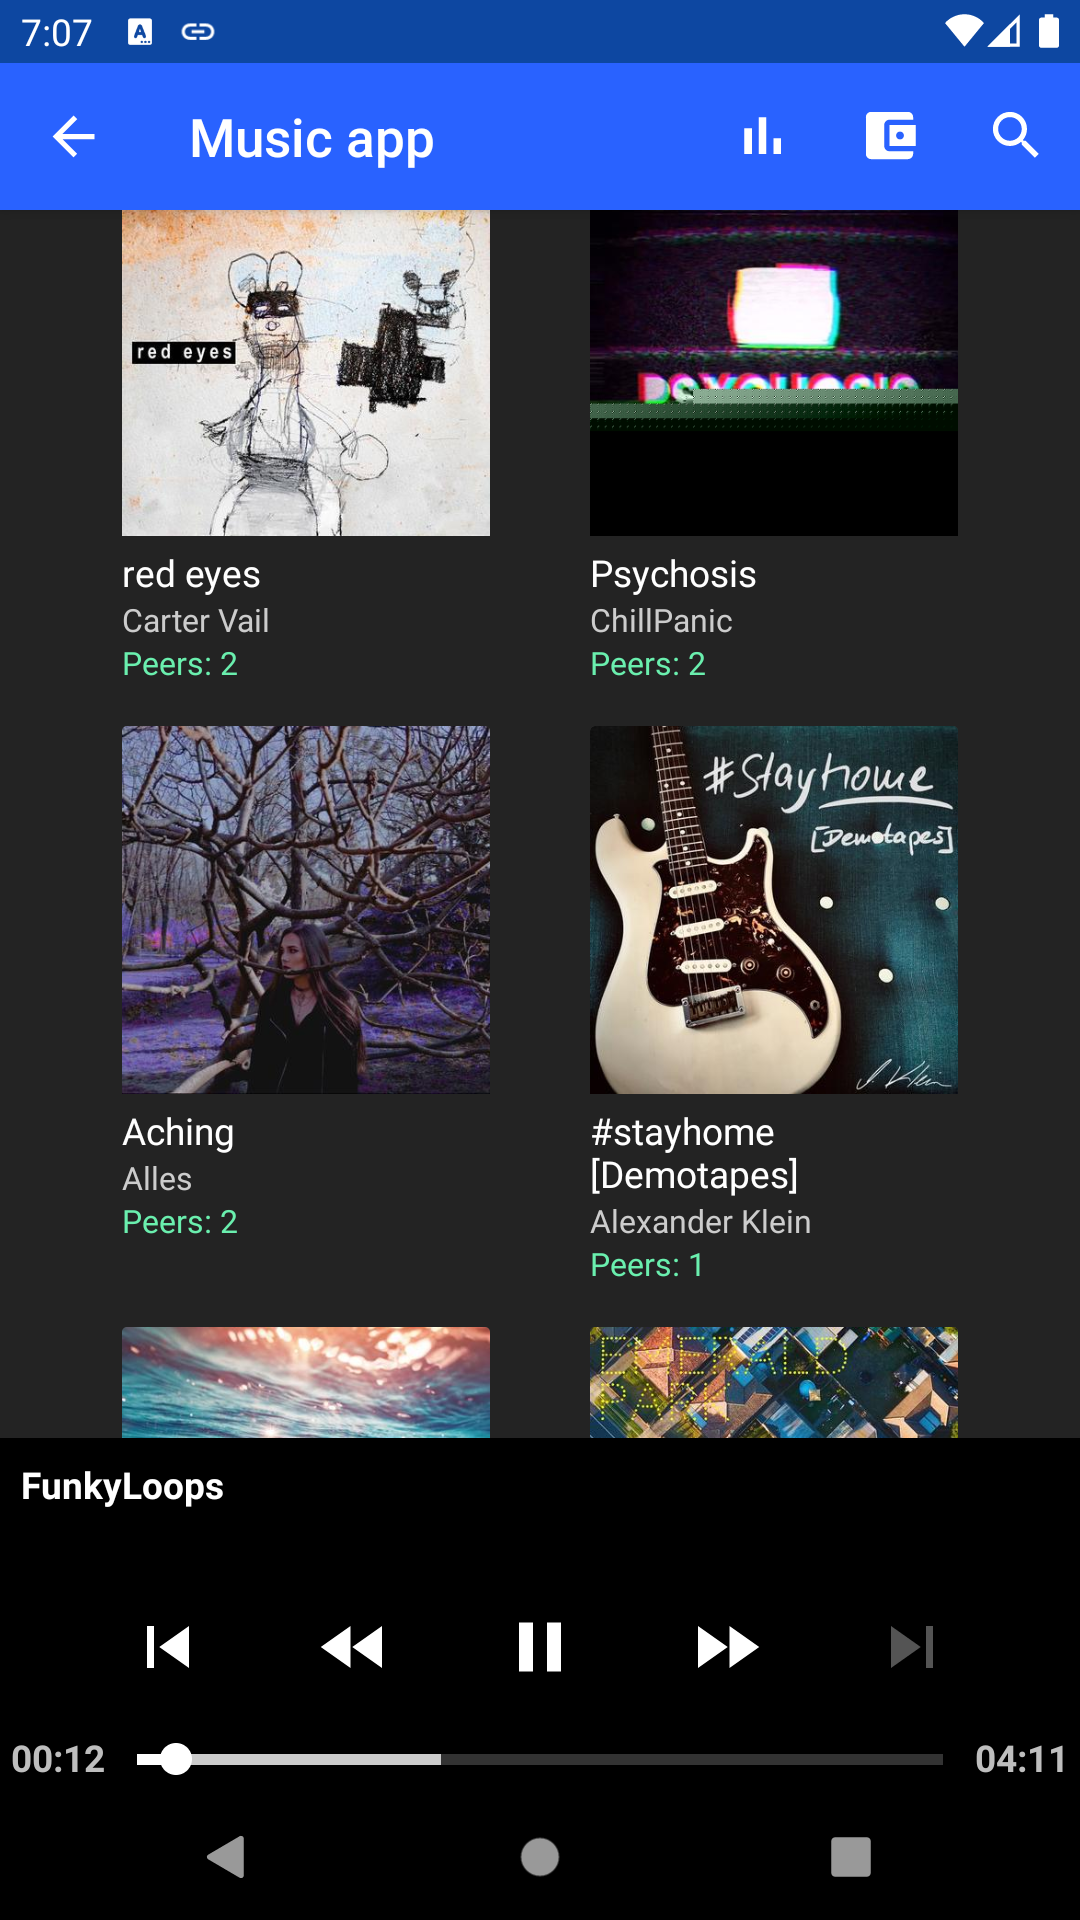
\includegraphics[width=1\linewidth]{implementation/overview.png}
        \caption{The playlist overview screen, which is the entrance screen}
        \label{fig:screenshot-home}
    \endminipage\hfill
    \minipage{0.3\textwidth}
        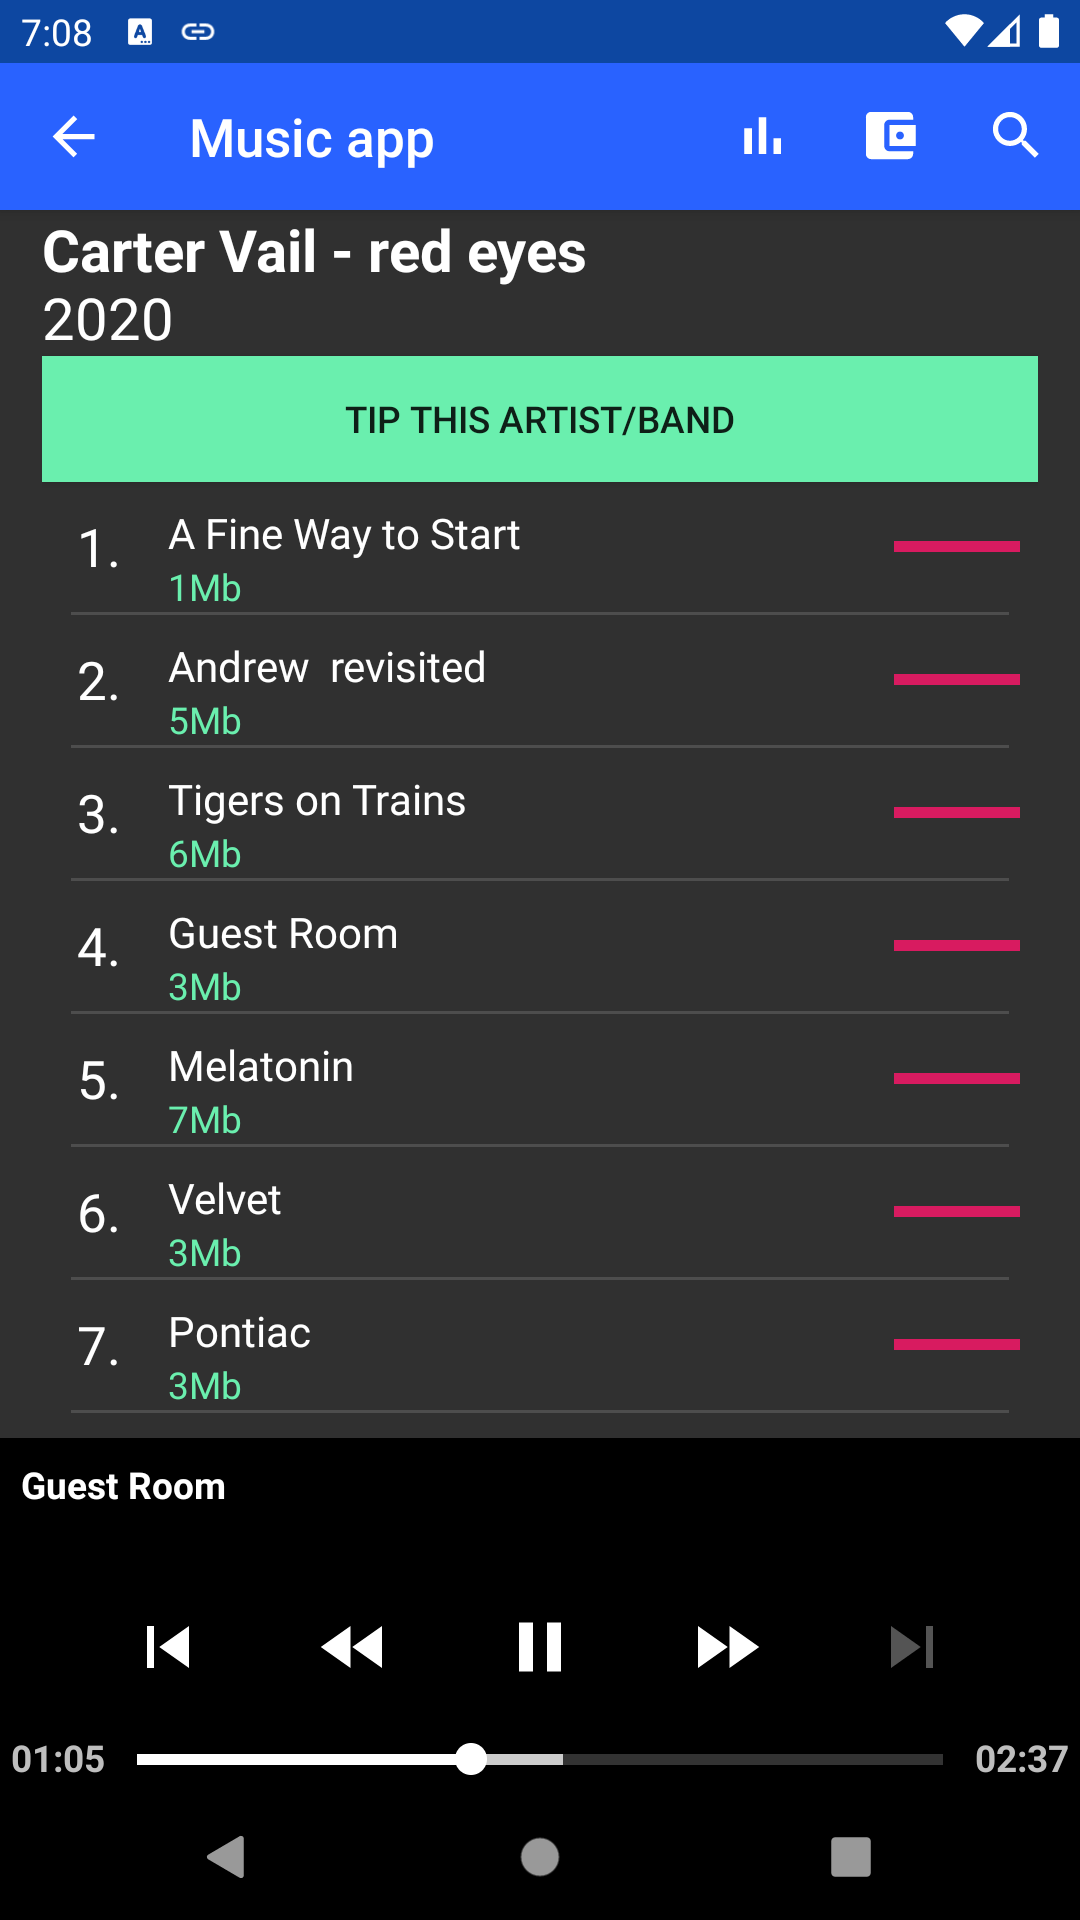
\includegraphics[width=1\linewidth]{implementation/playing-track.png}
        \caption{Playlist fragment, showing all tracks of one Release, streaming a track}
        \label{fig:screenshot-playlist}
    \endminipage\hfill
    \minipage{0.3\textwidth}
        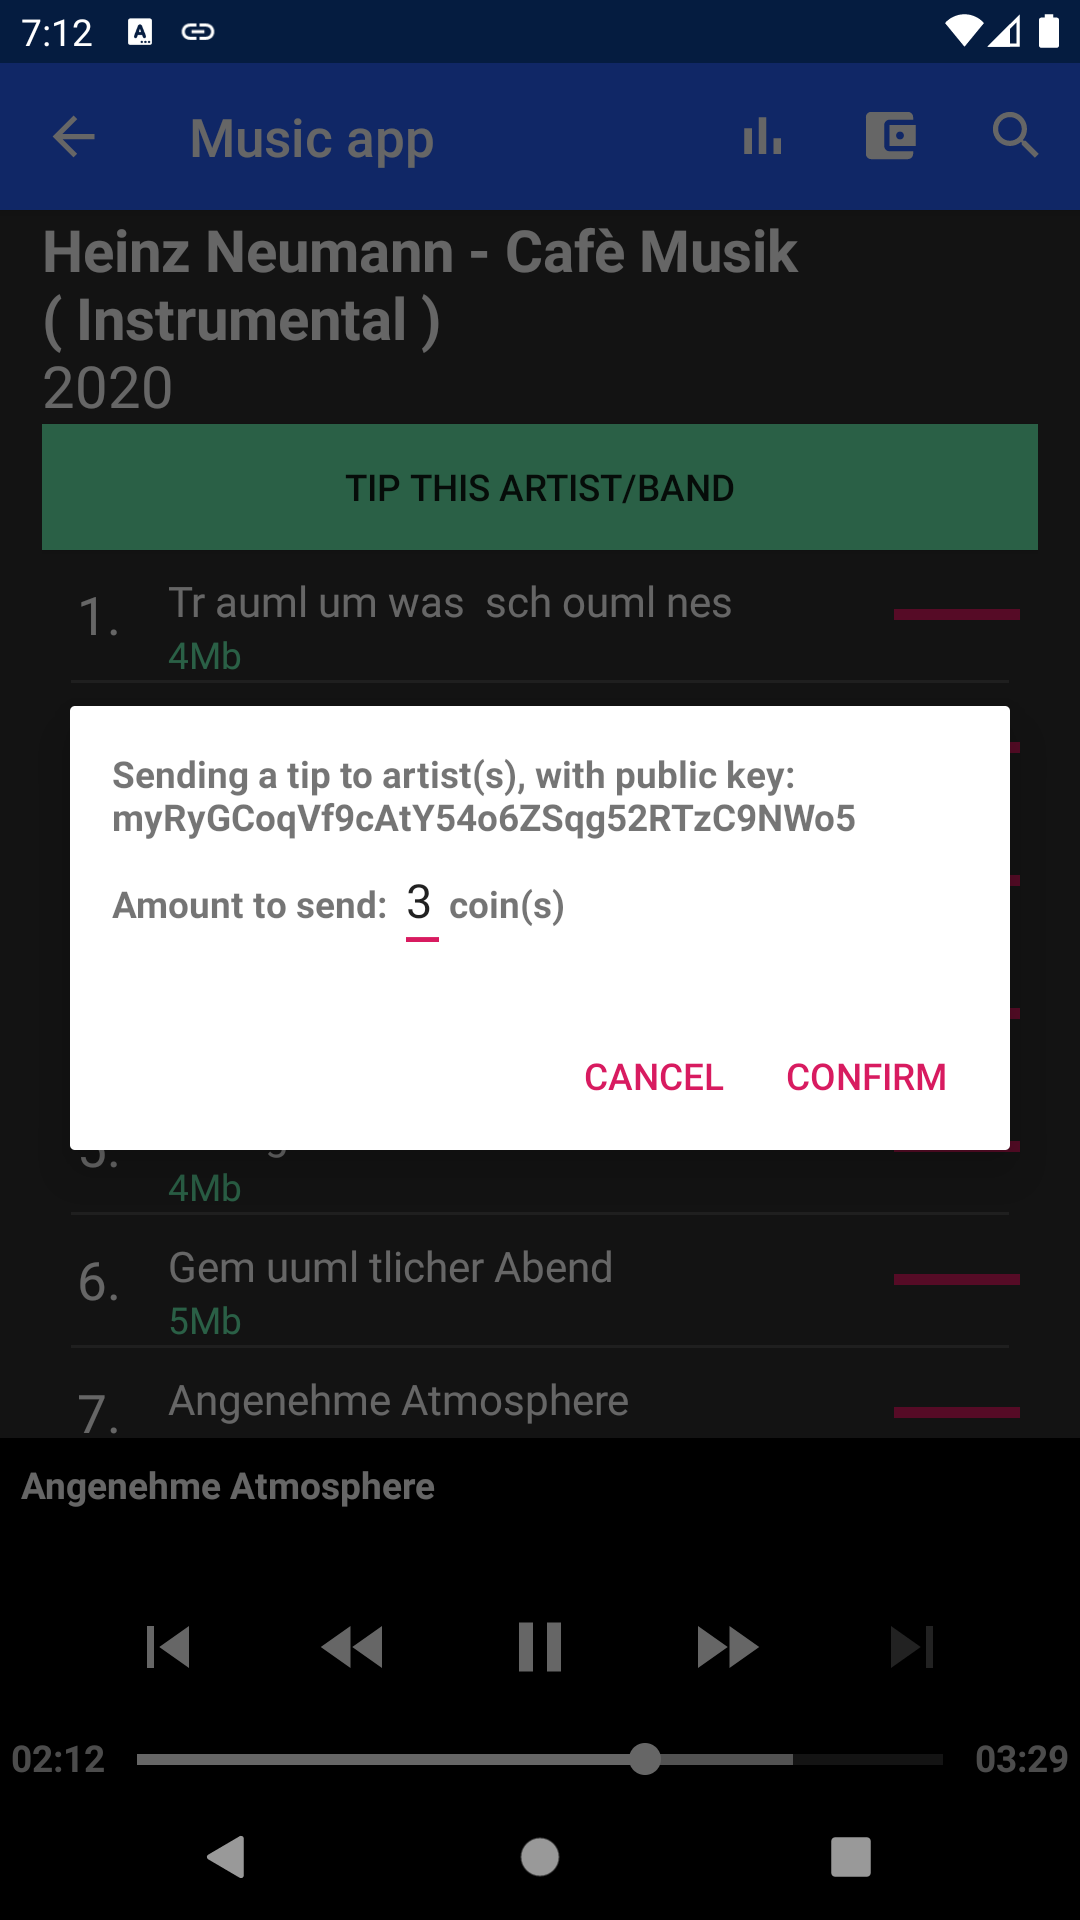
\includegraphics[width=1\linewidth]{implementation/send-tip}
        \caption{Sending a tip to an artist or band}
        \label{fig:tip-artist}
    \endminipage
\end{figure}

\section{Peer-to-peer content discovery}
Metadata discovery is implemented using push-based content spreading. Every $i$ seconds, every device sends a random block of music metadata to a random neighbor. 

The entry point of the app is the playlist overview screen (see fig. \ref{fig:screenshot-home}). It is the screen that is first shown upon starting the MusicDAO. Here the user is presented a list of playlists, with title and author, loaded from local disk and from peers. In our current implementation, each Playlist fragment corresponds to exactly one Release block (see fig. \ref{fig:release-model}). The playlists are sorted on their torrent swarm health in ascending order. Caching of audio files and metadata is used for fast browsing and music playback. The cover art shown in fig. \ref{fig:screenshot-home} is rendered using MP3 metadata processing. The system does not contain a pre-fetching mechanism for obtaining cover art (as observed in fig. \ref{fig:search-3}). Instead, it is only shown after at least one of the MP3 metadata has finished transferring using the BitTorrent stream.

% \subsection{Distributed keyword search algorithm}
\label{sec:searching-musiccommunity-impl}
MusicDAO allows users to search for music content remotely using keyword search. The search function tries to find matches locally, and if there are only a few found, it will try to ask for content from peers. Alg. \ref{alg:algorithm-distributed-search} is implemented using the parameters $ttl=1$ and $maxPeers=20$ so there is no recursive searching throughout the network. Any $ttl>1$ would result in an exponential message complexity. The current implementation uses only a simple filter, which checks if the keyword is contained in the metadata of the music release.

\begin{figure}
    \minipage{0.5\textwidth}
        \centering
        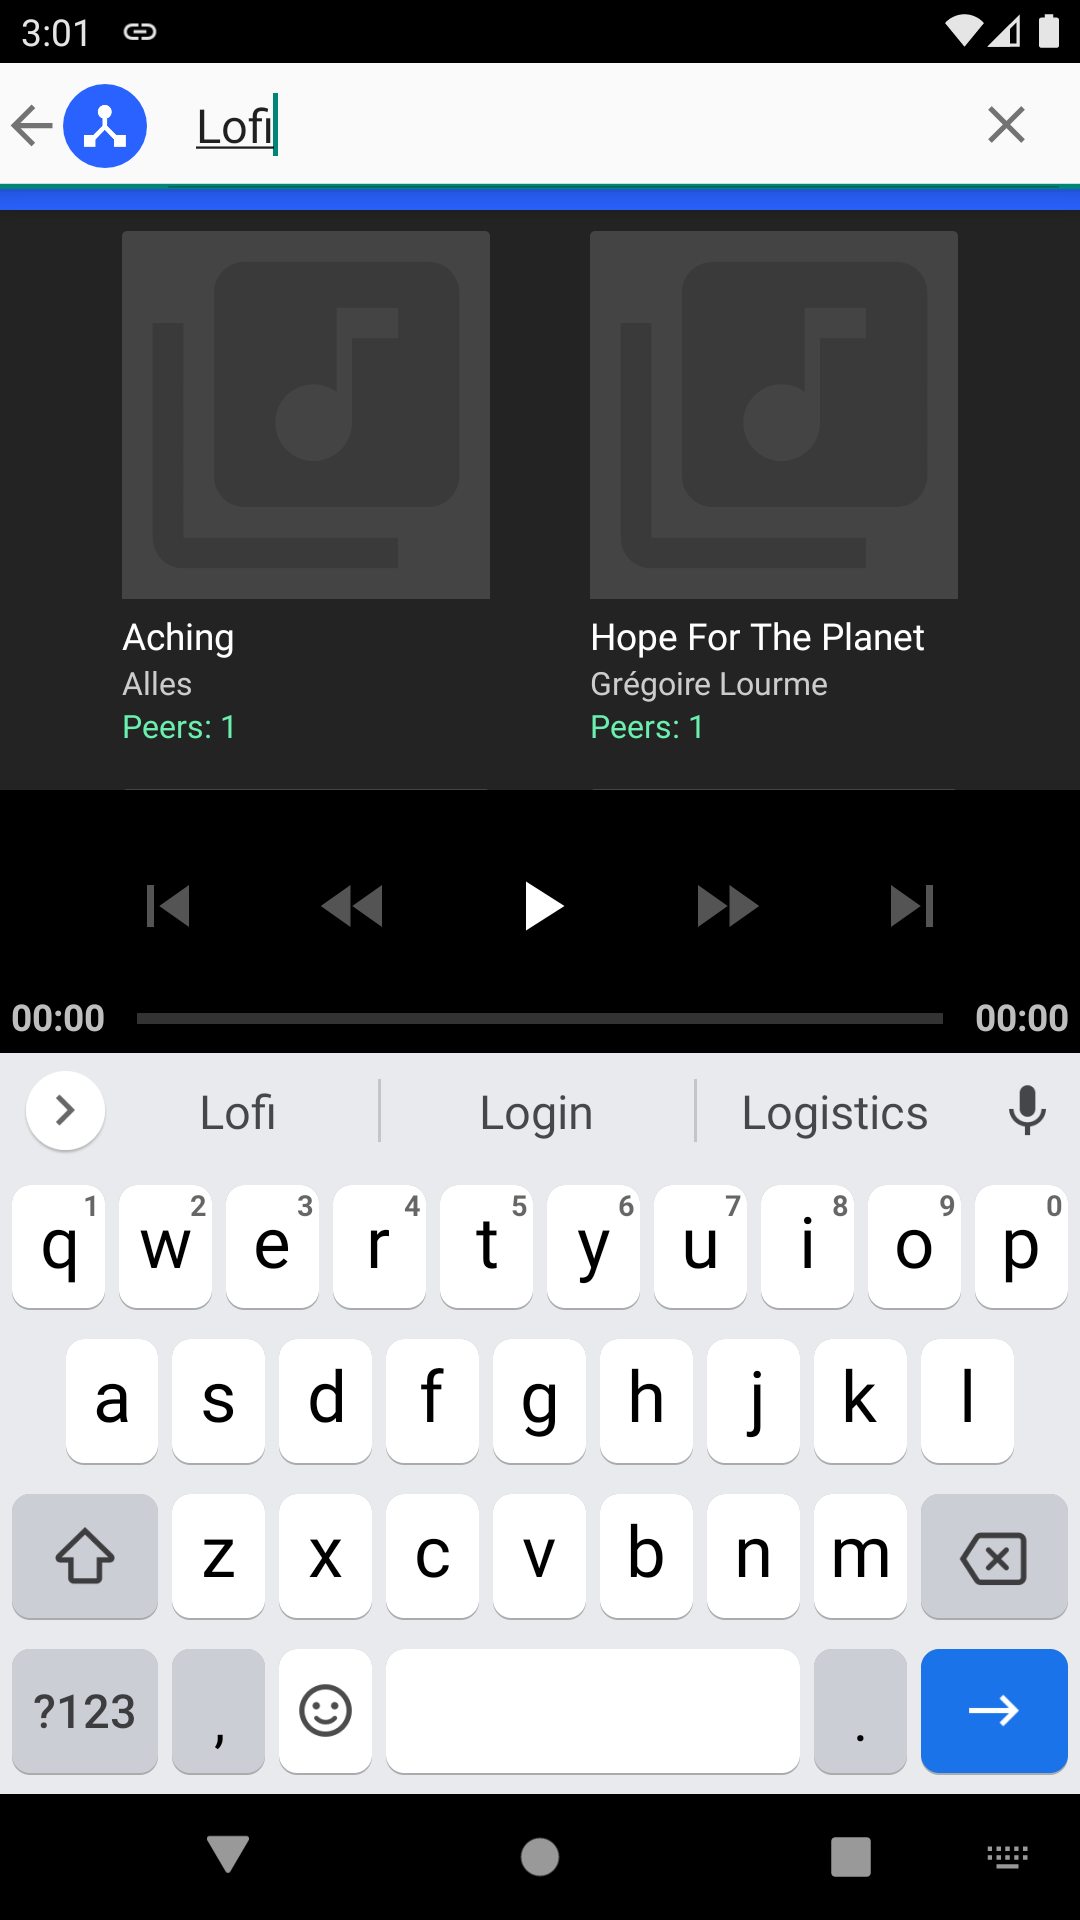
\includegraphics[width=0.6\linewidth]{implementation/search-2.png}
        \caption{Entering a search keyword}
        \label{fig:search-2}
    \endminipage\hfill
    \minipage{0.5\textwidth}
        \centering
        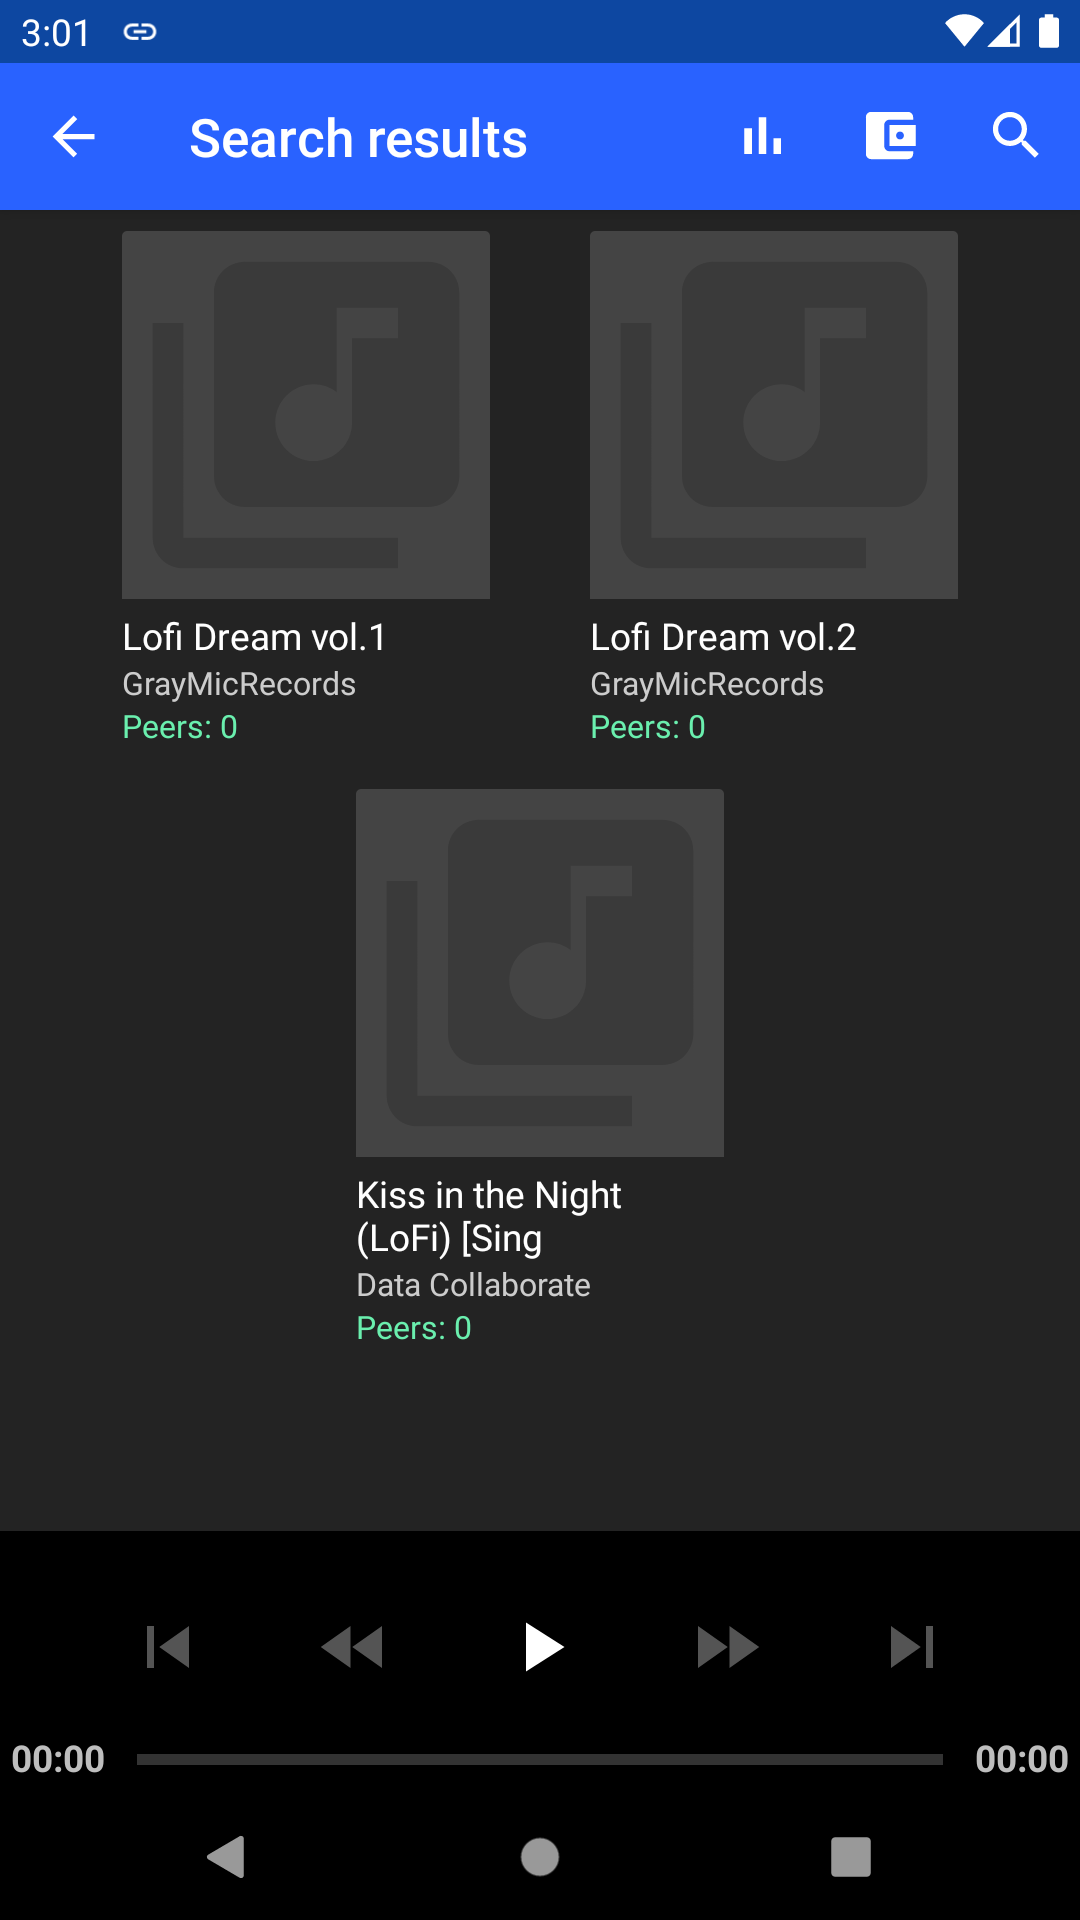
\includegraphics[width=0.6\linewidth]{implementation/search-3.png}
        \caption{Search results from peers, using keyword filtering}
        \label{fig:search-3}
    \endminipage\hfill
\end{figure}

% \subsection{Gossip-based content popularity algorithm}
The gossip-based algorithm used for communicating content popularity with peers is implemented as described in alg. \ref{alg:algorithm-content-popularity}. Every peer in the network sends a content health message to a random peer every 3 seconds. The content healthiness is displayed for every release as \textit{Peers: X} (see fig. \ref{fig:screenshot-home}). Gossip messages older than one hour are discarded ($margin=3600$).]

\section{Music streaming algorithm}
To be able to play music as soon as possible, we implemented a music streaming algorithm. It uses a priority system for tracks and for parts of tracks (chunks) (see \ref{fig:music-streaming-mechanism}). In essence, the player prioritizes chunks that the user is currently interested in, by actively asking peers to send the corresponding $k$ chunks that are necessary to play the selected section of the track. In addition, the selected track is given a higher priority over other tracks in the playlist. This uses the piece priorities system in libtorrent (see libtorrent Manual\footnote{\url{https://www.libtorrent.org/manual-ref.html\#file-format}}). By default, the first couple of chunks of each track are given a high priority, to reduce the chance of buffer underflow, so that the user can start streaming early. 
\begin{figure}
    \centering
    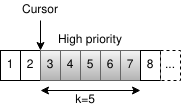
\includegraphics[width=0.25\textwidth]{implementation/streaming-algorithm.png}
    \caption{Music streaming mechanism}
    \label{fig:music-streaming-mechanism}
\end{figure}

Playing music is implemented using ExoPlayer\footnote{\url{https://github.com/google/ExoPlayer}}. This music player library is suitable as it allows for playing tracks that are partially loaded, which enables streaming. When the user selects a playlist to browse and play, the fragment in fig. \ref{fig:screenshot-playlist} is displayed. Here, the user can select a track to play. It presents its list of tracks and other metadata, such as the title and artist(s). For each track the file size is displayed, and a loading indicator on the right side. This shows, in real time, how much of the track is downloaded. In the example of \ref{fig:screenshot-playlist}, the first track is fully loaded. The track player, shown on the bottom, interacts directly with the tracklist and the selected track. It shows which track is selected and whether it is currently playing or buffering. 

\section{Peer-to-peer financial infrastructure}
\label{sec:regtest-network-impl}
Our system contains peer-to-peer payments where 100\% of money goes to artists. We created a public Bitcoin RegTest environment\footnote{\url{https://developer.bitcoin.org/examples/testing.html\#regtest-mode}} to test peer-to-peer Bitcoin donations and payments. This creates a new `clean slate' Bitcoin blockchain and allows for full control over the chain and miners. This enables a test environment that is useful for experiments, as we can tweak the block generation speed and keep track of all transactions registered on the blockchain.

Each device participating in the MusicCommunity is given a private/public wallet identity upon installation of the MusicDAO. The wallet interface (fig. \ref{fig:wallet-sync}) shows synchronization status of the blockchain. Once the wallet is fully synchronized with the blockchain, the private key and balance are displayed as shown in fig. \ref{fig:wallet-balance}. 

Each device must be synchronized with the network in order to make payments. A background thread of MusicDAO establishes and maintains communication with bitcoin nodes, so that it does not interrupt the user experience. Synchronization with the RegTest network is done using a single bootstrap server, which is a hard-coded address in the app. This is necessary for running on a test net, as it will take an infeasible amount of time to guess the address of a running Bitcoin node, with only a few nodes. In a real-world situation, bitcoin nodes should be found by querying peers for bitcoin node addresses.

Upon browsing a playlist, a donation button is displayed as shown in fig. \ref{fig:tip-artist}. The user can select an amount and make a direct donation to the artist or band, in the form of a bitcoin transaction from their wallet. All transactions are atomic, so an automated splitting system between e.g. artists in a band could be a logical extension.
\begin{figure}
    \minipage{0.3\textwidth}
        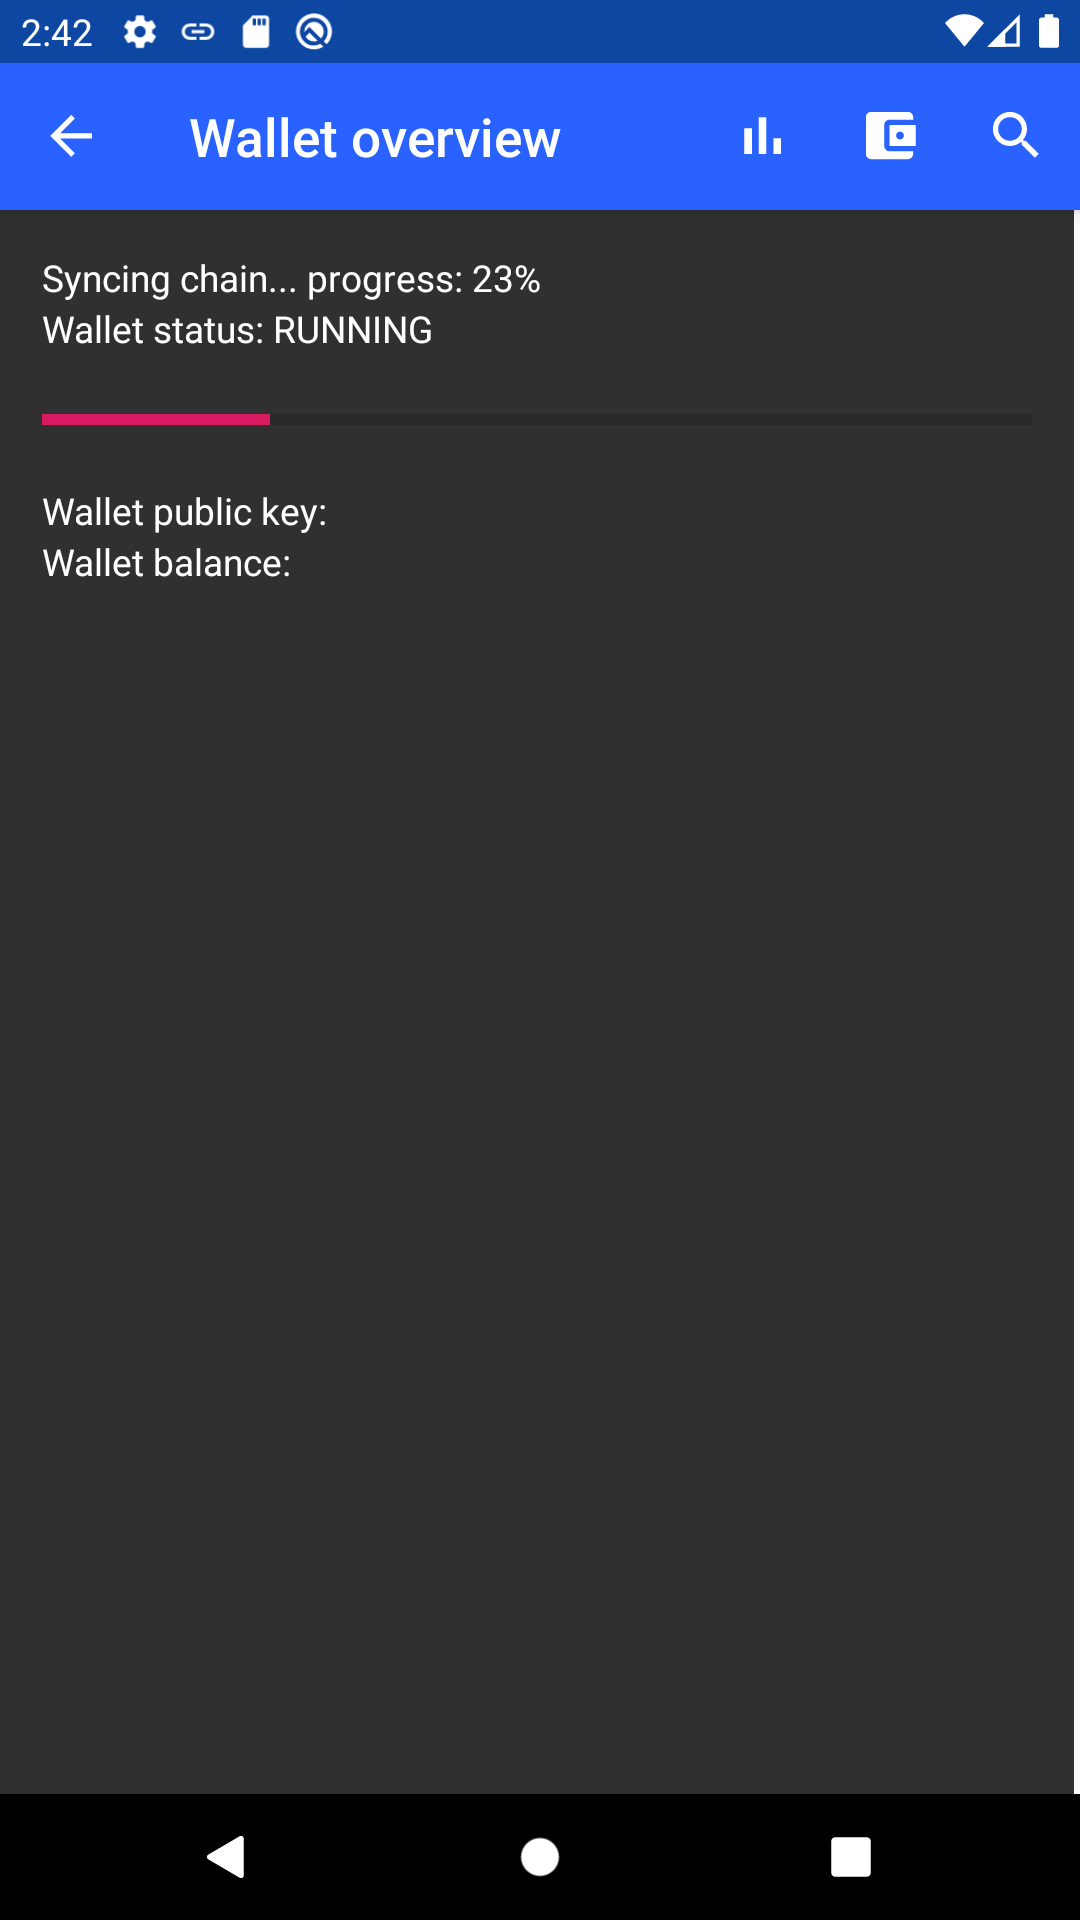
\includegraphics[width=1\linewidth]{implementation/wallet-sync.png}
        \caption{Synchronizing the Bitcoin RegTest environment blockchain}
        \label{fig:wallet-sync}
    \endminipage\hfill
    \minipage{0.3\textwidth}
        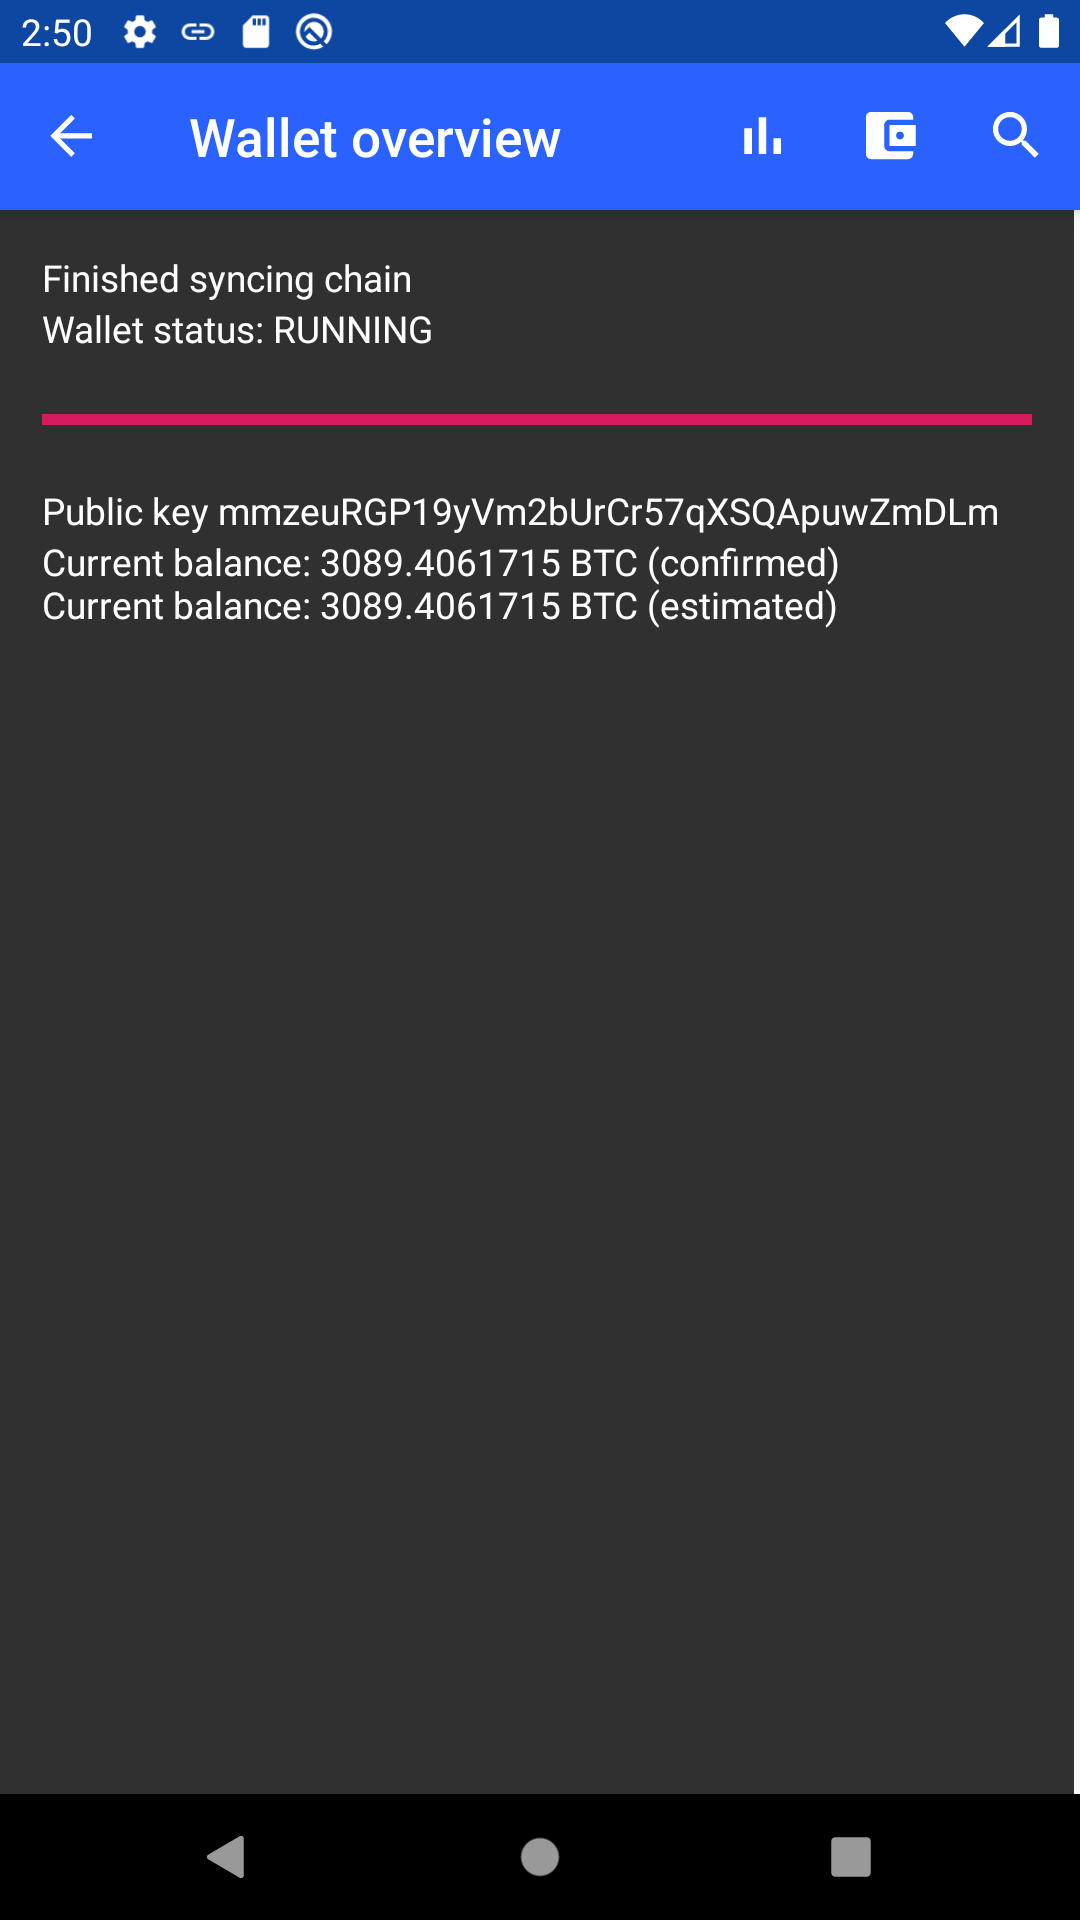
\includegraphics[width=1\linewidth]{implementation/wallet-balance.png}
        \caption{Wallet overview and balance after synchronizing}
        \label{fig:wallet-balance}
    \endminipage\hfill
    \minipage{0.3\textwidth}
        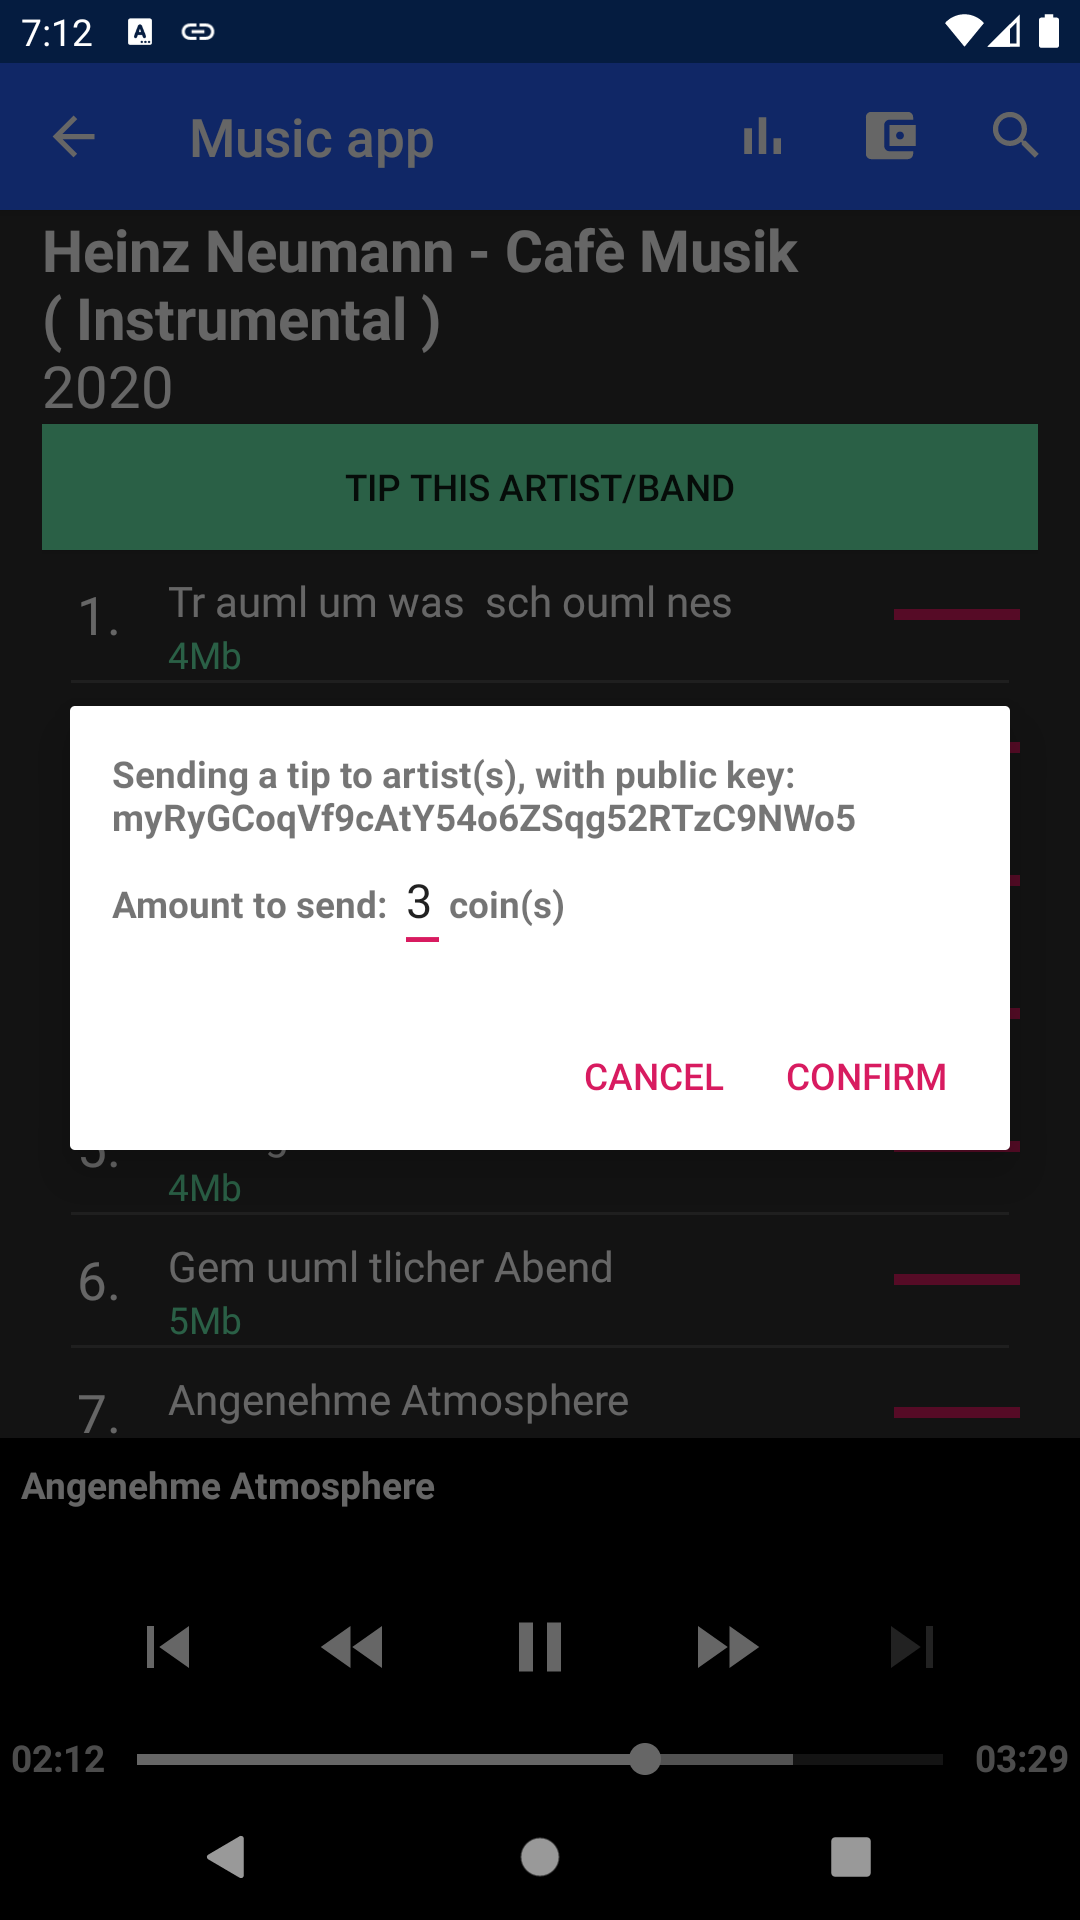
\includegraphics[width=1\linewidth]{implementation/send-tip.png}
        \caption{Sending a tip to an artist or band}
        \label{fig:tip-artist}
    \endminipage\hfill
\end{figure}

\section{Self-publishing of music}
We implement audio track uploading, downloading and streaming using JLibtorrent\footnote{\url{https://github.com/frostwire/frostwire-jlibtorrent}}, an implementation of BitTorrent. Immutable and public storage of metadata is implemented with TrustChain~\citep{otte2017trustchain}. 
% This technology has shown to run well on mobile devices (cite), and allows for extensive configuration.
\label{sec:torrent-creation}
To create and share music content, a user can create a Release object using the dialog shown in fig. \ref{fig:submit-release-dialog}. Releases can be made by selecting local audio tracks or a magnet link. 

We run a BitTorrent tracker, which maintains a list of seeders for the torrents that are created and shared in MusicDAO. To keep the network decentralized, seeders may also be found using a distributed hash table~\citep{bittorrentbep5dht}. In addition, the app uses the local peer discovery (LPD)~\citep{bittorrentbep142015} functionality of BitTorrent. This allows for finding peers and transmitting torrent pieces over a LAN, resulting in fast transmission and low latency.
\label{sec:content-seeding}
Seeding of content is implemented using a simple continuous mechanism. The ContentSeeder class runs a background thread and seeds torrents using a first-in-first-out heuristic: $K\leq 5$ most recent torrents are seeded.

\begin{figure}
    \centering
    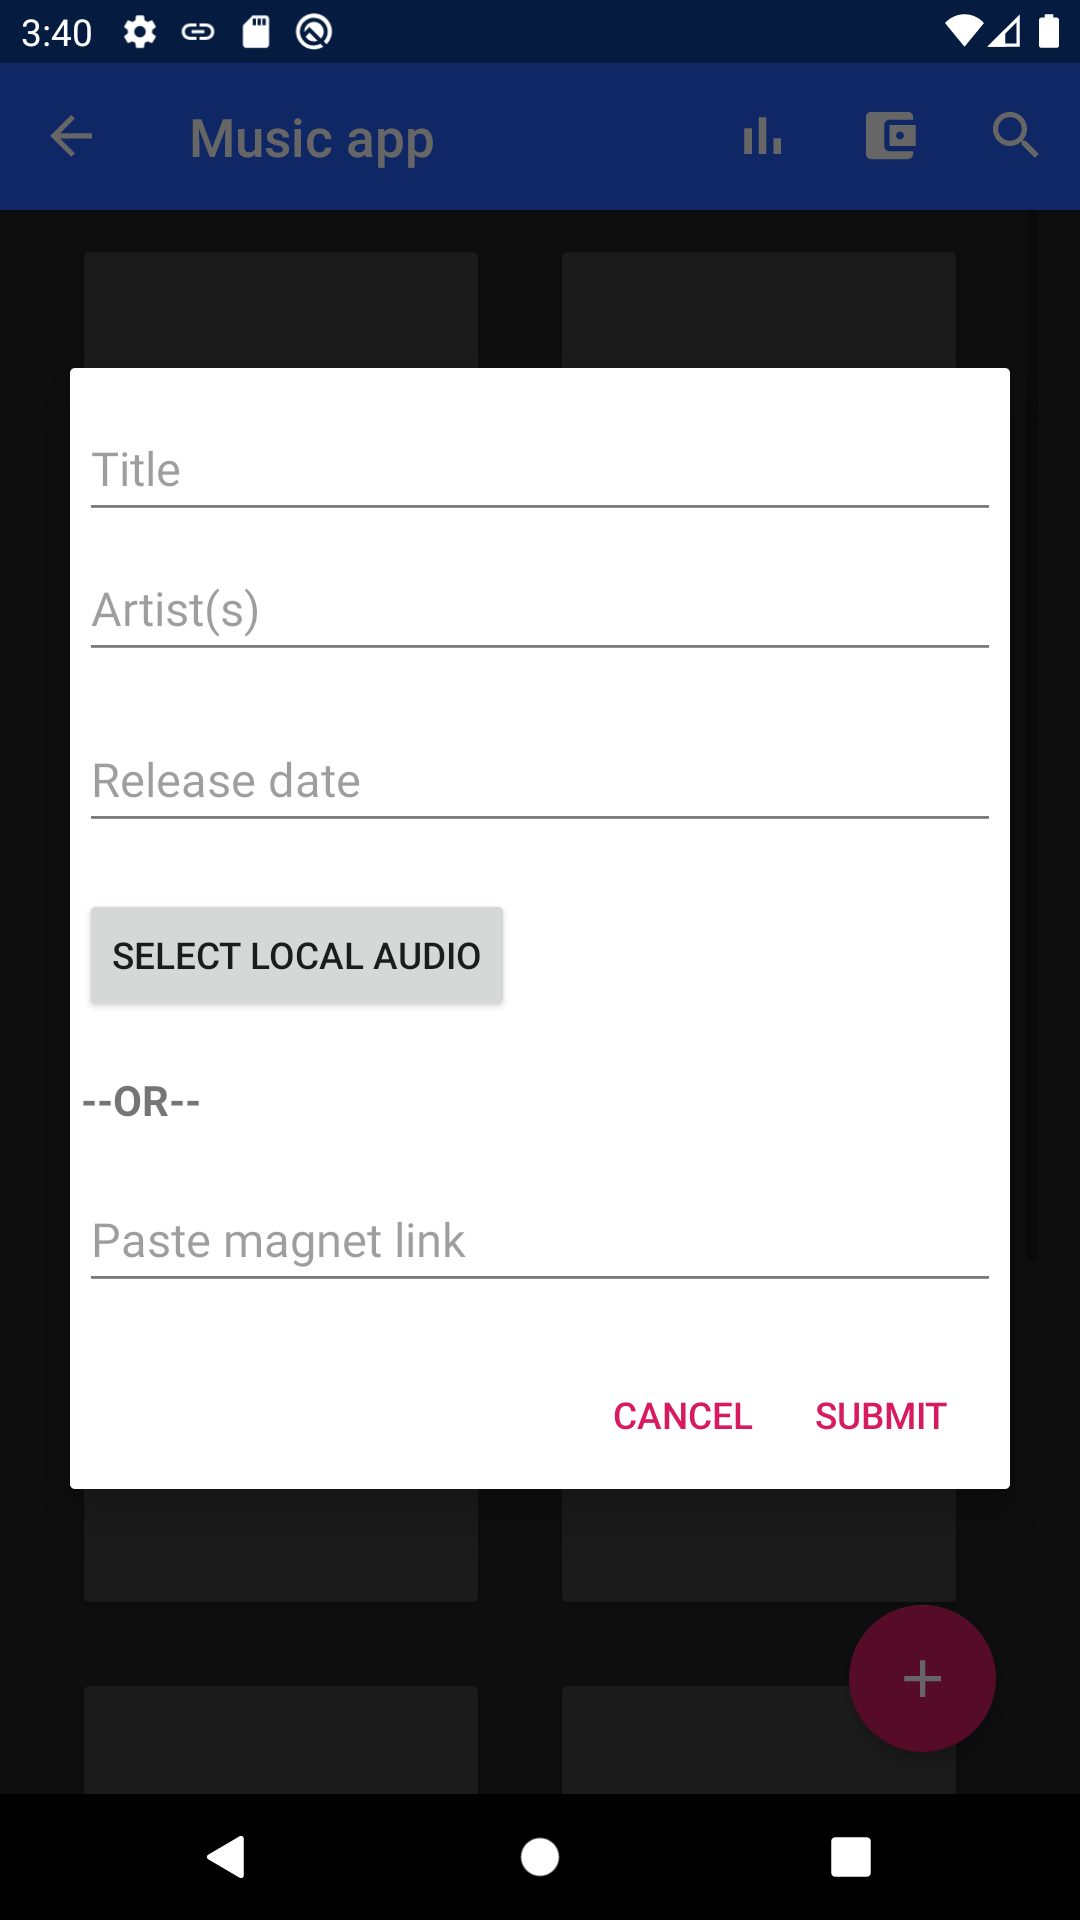
\includegraphics[width=0.3\textwidth]{implementation/screenshot-select-tracks.png}
    \caption{Dialog for creating and publishing a new Release}
    \label{fig:submit-release-dialog}
\end{figure}

\section{Identity and authenticity}
\label{sec:identity-authenticity}
Every device participating in MusicDAO has a unique identity. MusicDAO implements the public-key infrastructure as described in \ref{sec:pki-design} using the identity system proposed by \cite{mattskala2020}. This uses the widely used industry standard Curve25519 cryptography system. Using this system, it is computationally infeasible to obtain the private key from a  public key. For simplicity in implementation, we assume that every device in the network is an abstraction of a unique artist.

All immutable music release blocks are assigned an identity of the creator using a public key. Every device running the MusicDAO will receive a public/private key-pair upon first launch. 

Currently there is no multi-signature support implemented. This means that in the case of a group publishing a Release, there is only one public key representing the whole group. Every artist, and every unique collaboration between artists should generate their own key-pair to describe ownership of the Release.

\section{Quality assurance}
As mentioned in the introduction, the goal of the implemented work is to be the first steps towards a full robot economy. Aside from being a functional real-world application, its implementation contains key components from our framework that can be reused to implement robot economy software for other domains. Experimentation in other domains allows to gain a further understanding of the developing science of the robot economy. This means software reusability is of great importance in our work. Therefore we use code quality assurance best practices such as continuous integration, code linting and pull request reviews. These best practices are widely used in the software industry. 

We use a continuous integration (CI) environment, run by Github Actions\footnote{\url{https://github.com/features/actions}}. GitHub Actions is a mature CI system, used by e.g. the Google Cloud Platform. Within our CI environment, we use automated tests and code linting. Unit tests are written using JUnit 4\footnote{\url{https://junit.org/junit4/}} and the mocking library Mockk\footnote{\url{https://mockk.io/}}. The code coverage of these unit tests can be seen in \ref{tab:code-cov}. Code linting is performed using KtLint\footnote{\url{https://github.com/pinterest/ktlint}}. For every 100 lines of code, there are around 17 lines of documentation.

Code coverage is measured by Android Studio 4\footnote{\url{https://developer.android.com/studio}}. The majority of uncovered code contain user interface interaction and networking callback logic. Code coverage could have been improved by introducing integration tests (using Android instrumented tests). These are tests that run on an Android device or emulator so that user interaction flows can be tested. 

MusicDAO runs on Android 5.1.1 and above, and as such supports 13,734 different Android devices\footnote{According to Google Play Console, 17-02-2021.}. During the implementation phase we ensure that it runs well on different screen sizes and Android versions, by running it on 10 different Android devices. To gain a further understanding of device compatibility and bug hunting, we make use of an online crash reporter (fig. \ref{fig:firebase-crashlytics}). Firebase Crashlytics\footnote{\url{https://firebase.google.com/docs/crashlytics}} registers app installs and crashes in real-time, which we use during the experimentation of MusicDAO. It shows details of each application crash for all users (see fig. \ref{fig:firebase-crashlytics}). Using this, a full stack trace can be inspected remotely for each crash. In addition it helps with gaining insight in various performance metrics for certain types of Android devices.

% The code-base contains 1 line of documentation for 10 lines of code

\begin{table}[]
\centering
\begin{tabular}{|l|l|l|l|}
\hline
\textbf{Package/class} & \textbf{Line coverage} & \textbf{Lines of code} \\ \hline
MusicService.kt        & 27\%   & 207         \\ \hline
MusicBaseFragment.kt   & 50\%  & 11            \\ \hline
MusicGossipingService.kt & 41\% & 75          \\ \hline
catalog                & 20\% & 249          \\ \hline
dialog                 & 9\% & 142          \\ \hline
ipv8                   & 92\% & 229          \\ \hline
net                    & 71\% & 109          \\ \hline
player                 & 0\% & 80             \\ \hline
playlist               & 3\% & 346           \\ \hline
util                   & 69\% & 224              \\ \hline
wallet                 & 36\% & 199           \\ \hline
\textbf{Total} & \textbf{37\%} & \textbf{1871} \\ \hline
\end{tabular}
\caption{Code coverage overview}
\label{tab:code-cov}
\end{table}

% Replace with newer version of this image showing 94% crash-free users
\begin{figure}
    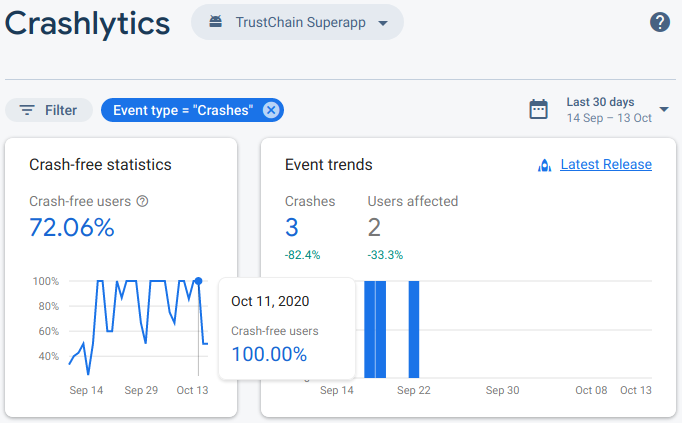
\includegraphics[width=0.7\linewidth]{implementation/firebase-crashlytics.png}
    \caption{Firebase Crashlytics crash reporter; this figure shows the crashes over time}
    \label{fig:firebase-crashlytics}
\end{figure}